\documentclass{beamer}
\usepackage[utf8]{inputenc}
\usepackage[czech, english]{babel}

\usetheme{Warsaw}
\title[Demonstrační aplikace pro podporu kurzu neuronových sítí]{Demonstrační aplikace pro podporu kurzu neuronových sítí}
\author{Adam Činčura}
\institute{ČVUT - FEL}
\date{28. 6. 2011}
\defbeamertemplate*{footline}{shadow theme}
{%
  \leavevmode%
  \hbox{\begin{beamercolorbox}[wd=.47\paperwidth,ht=2.5ex,dp=1.125ex,leftskip=.3cm plus1fil,rightskip=.3cm]{author in head/foot}%
    \usebeamerfont{author in head/foot}\insertshortauthor
  \end{beamercolorbox}%
  \begin{beamercolorbox}[wd=.53\paperwidth,ht=2.5ex,dp=1.125ex,leftskip=.3cm,rightskip=.3cm plus1fil]{title in head/foot}%
    \usebeamerfont{title in head/foot}\insertshorttitle\hfill\insertframenumber\,/\,\inserttotalframenumber%
  \end{beamercolorbox}}%
  \vskip0pt%
}

%\setbeamertemplate{footline}[page number]
\begin{document}

\begin{frame}
\titlepage
\end{frame}
\section{Úvod}
\begin{frame}{Obsah}
   \tableofcontents
\end{frame}
\begin{frame}{Zadání}

\begin{itemize}
\item Zadání:

Seznamte se s elektronickou přílohou skript pro předmět "neuronové sítě a neuropočítače" - tzv. courseware. Rozšiřte tento soubor o demonstrační aplikace v systému Wolfram Mathematica s využitím aplikační knihovny NeuralNetworks. Formu a konkrétní aplikace zvolte po dohodě s vedoucím práce. Výsledky práce budou použity ve výuce.


\item Vedoucí práce: Ing. Zdeněk Buk
\item Oponent: Ing. Miroslav Čepek
\end{itemize}
\end{frame}

\begin{frame}{Cíle práce}
\begin{itemize}
\item Rozšíření elektronické přílohy skript Neuronové sítě a neuropočítače - Courseware
\item Vytvořit podpůrný materiál pro výuku (36NAN, Y336VD)
\item Umožnit studentům snadné experimentování s neuronovými sítěmi
\item Pomocí interaktivních příkladů přiblížit fungování sítí
\end{itemize}

\end{frame}

\begin{frame}{Struktura práce}
\begin{itemize}
\item Demonstrační aplikace
\item Teoretická část
\item HTML stránka
\end{itemize}
\end{frame}


\section{Demonstrační aplikace}
\begin{frame}{Demonstrace principu neuronové sítě}
\begin{itemize}
\item Slouží k pochopení vnitřní funkcionality sítě a učicích algoritmů
\end{itemize} 
  \begin{columns}[T]
    \column{5cm}
      \begin{figure}
   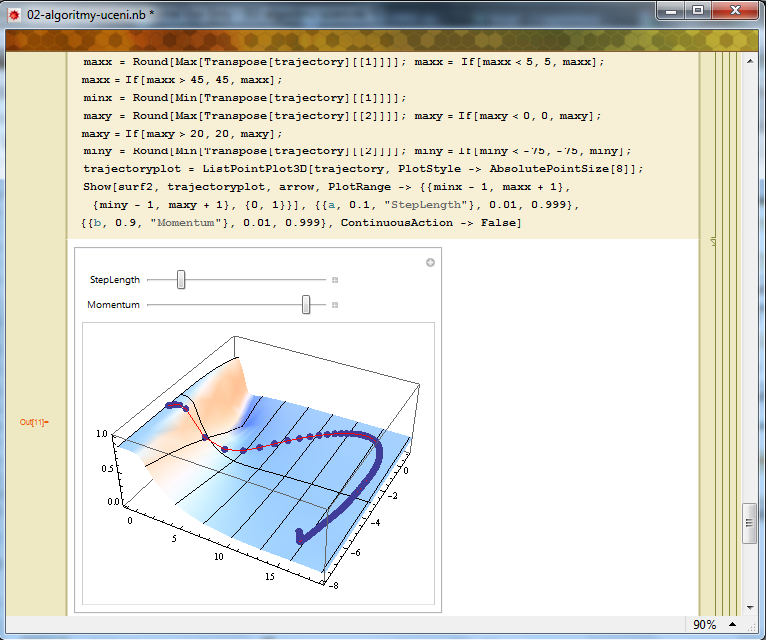
\includegraphics[width=5.5cm]{uk1.png}
\end{figure}
    \column{5cm}
      \begin{figure}
   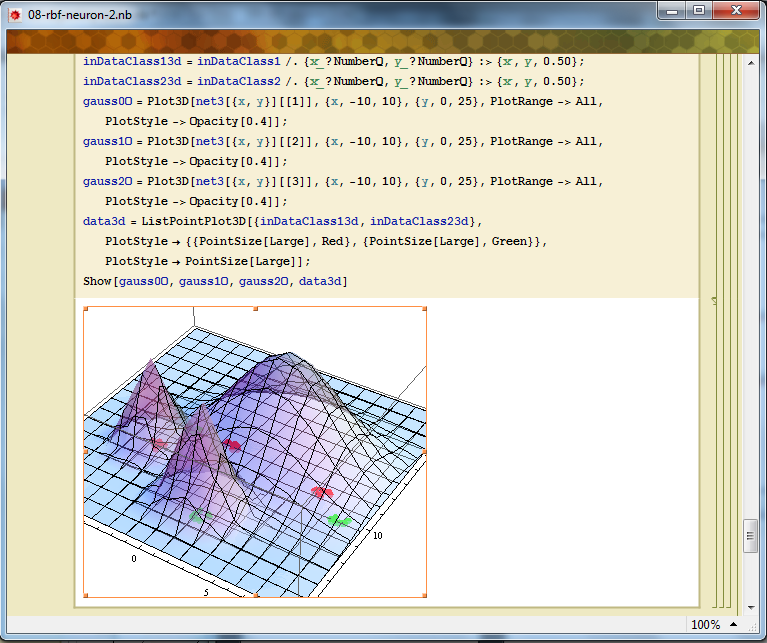
\includegraphics[width=5.5cm]{uk2.png}
\end{figure}
  \end{columns}
\end{frame}


\begin{frame}{Demonstrace použití neuronové sítě}
\begin{itemize}
\item Demonstrují vytváření a jednoduchou práci s neuronovými sítěmi
\end{itemize} 
  \begin{columns}[T]
    \column{5cm}
      \begin{figure}
   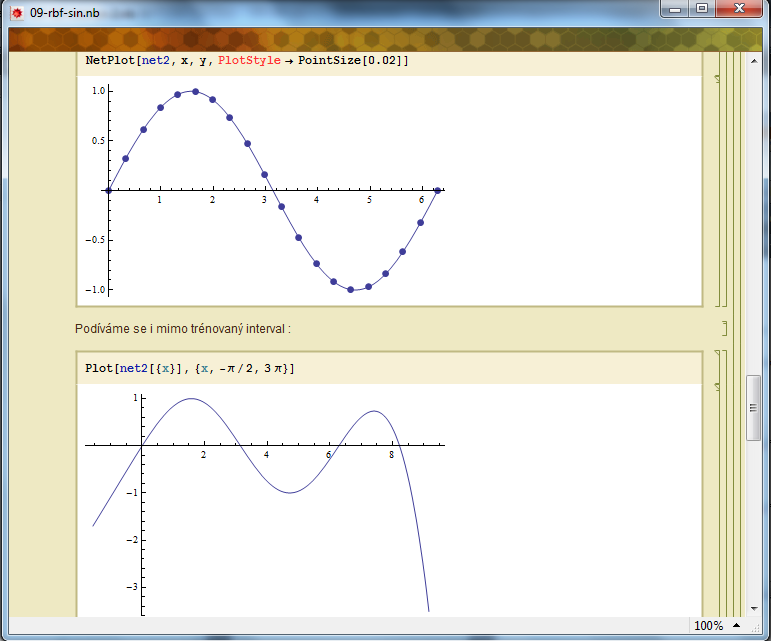
\includegraphics[width=5.5cm]{uk3.png}
\end{figure}
    \column{5cm}
      \begin{figure}
   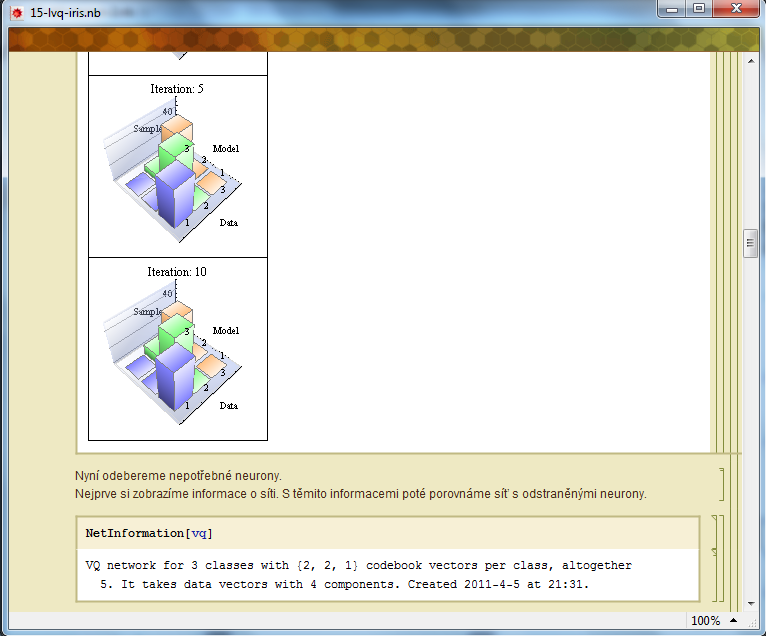
\includegraphics[width=5.5cm]{uk4.png}
\end{figure}
  \end{columns}
\end{frame}

\begin{frame}{Demonstrace vyhodnocení neuronové sítě}
\begin{itemize}
\item Ukazují jakými způsoby zhodnotit výstup sítě
\end{itemize} 
  \begin{columns}[T]
    \column{5cm}
      \begin{figure}
   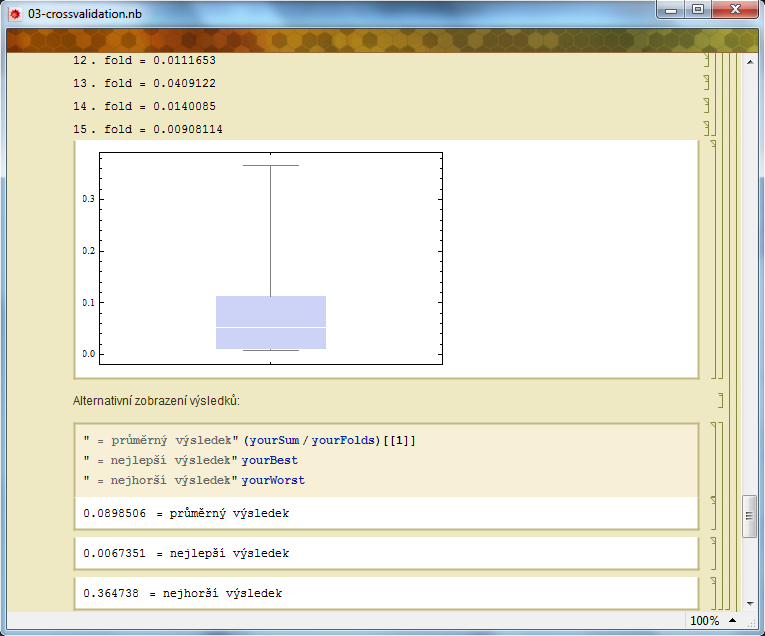
\includegraphics[width=5.5cm]{uk5.png}
\end{figure}
    \column{5cm}
      \begin{figure}
   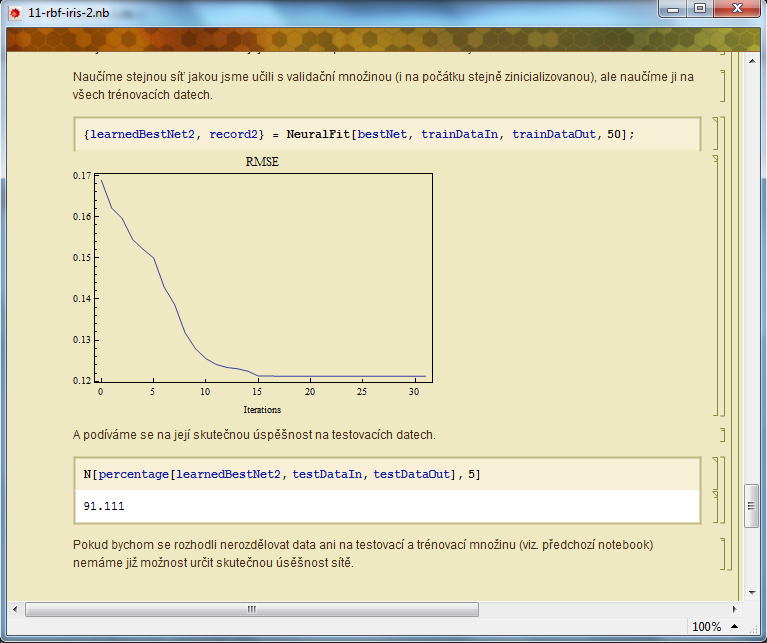
\includegraphics[width=5.5cm]{uk6.png}
\end{figure}
  \end{columns}
\end{frame}

\begin{frame}{Původní demonstrační aplikace}
\begin{itemize}
\item Autorem Petr Chlumský
\item Z roku 2008
\item Obsahovala 8 interaktivních souborů
\item Pokrývala základní použití neuronových sítí
\end{itemize}
\end{frame}
\begin{frame}{Nová demonstrační aplikace}
\begin{itemize}
\item 15 interaktivních souborů
\item Mezi nimi i přepracované soubory z původní aplikace
\item Rozšiřuje původní aplikaci hlavně o:
\begin{itemize}
\item Porovnání různých učicích algoritmů u dopředných sítí
\item Vyhodnocení úspěšnosti sítě pomocí křížové validace
\item Možnost určení úspěšnosti sítě v procentech
\item Příklady učení sítě s využitím trénovací, testovací a validační množiny
\item Demonstraci fungování RBF sítě
\item Ukázku průběhu učení samoorganizující se mapy
\end{itemize}
\end{itemize}
\end{frame}


\section{Teoretická část práce}
\begin{frame}{Teoretická část práce}
\begin{itemize}
\item Historický úvod do problematiky neuronových sítí
\item Popis neuronu a jeho fungování
\item Popis neuronových sítí včetně jejich algoritmů učení. Konkrétně jsou popsány:
\begin{itemize}
\item Dopředná síť
\item RBF síť
\item Hopfieldova síť
\item Samoorganizující mapa
\item LVQ síť
\end{itemize}
\item Popis křížové validace
\end{itemize}
\end{frame}
\section{Vývojové prostředí}
\begin{frame}{Wolfram Mathematica}
\begin{itemize}
\item Sofistikovaný systém pro matematické výpočty
\item Široké možnosti vizualizace dat
\item Rozšiřitelné o velké množství knihoven 
\item Použita verze 8.0
\end{itemize}

\end{frame}

\begin{frame}{Knihovna Neural Networks}
\begin{itemize}
\item Autorem Jonas Sjöberg 
\item Implementuje základní neuronové sítě
\item Implementuje učicí algoritmy pro jednotlivé sítě
\item Nabízí základní možnosti vizualizace sítí
\item Použita verze 1.1.0.0, později verze 1.1.2
\end{itemize}
\end{frame}
\begin{frame}{Zhodnocení práce}
\begin{itemize}
\item Splněny cíle práce
\item Aplikaci je možné okamžitě použít ve výuce
\end{itemize}
\end{frame}


\begin{frame}{Závěr}
\begin{center}
\begin{huge}
Děkuji za pozornost.
\end{huge}
\end{center}

\end{frame}
\end{document}